%! TEX root = ../main.tex
\section{Evolución}
\label{sec:tics_educacion}

Todas las prácticas educacionales están basadas en asunciones filosóficas acerca
de la naturaleza de los estudiantes, y los mecanismos que permiten al ser humano
aprender\cite{johnson2005instructionism}.

La utilización actual de las \Gls{tic} en la educación no es un fenómeno
asilado, responde a una evolución constante de la tecnología y metodología
utilizada.

Desde sus inicios, existieron varias corrientes pedagógicas que utilizaron en
mayor o menor medida a las \Gls{tic}, desde ser utilizada como una herramienta
para suplantar a libros impresos, proyectores,
etc\cite{nanjappa2003constructing}; hasta como una herramienta de aprendizaje
de pensamiento de alto
nivel\cite{egenfeldt2007third,white:ict,nanjappa2003constructing}.

De las diferentes pedagogías existentes, existen cuatro en la que las \Gls{tic}
han sido utilizadas de manera activa, las cuales son el instruccionismo o
educación tradicional, el conductismo, el constructivismo y finalmente, el
construccionismo. Esto no implica que las \Gls{tic} no puedan ser aplicadas
a otras pedagogías, es más, existen otras corrientes que utilizan las \Gls{tic},
de diversas maneras como el cognoscitivismo\cite{egenfeldt2007third} y el
conectivismo\cite{white:ict}. 

Cada corriente pedagógica utiliza las \Gls{tic} de manera diferente, sí bien
comparten características, no deben ser consideradas como una sucesión de
pedagogías que desembocan en una pedagogía utilizada actualmente.

\subsection{Antecedentes}

La historia de las \Gls{tic} en educación comienza en la \enquote{Open
    University of United Kingdom} que en $1969$ se establece como la primera
institución educativa dedicada a la enseñanza a distancia utilizando las, para
aquel entonces, nuevas tecnologías\cite{tinio:ict}. 

El análisis de la historia de las \Gls{tic} en educación es indispensable,
aunque existe una corriente que tiende a desestimar las experiencias pasadas,
cuyo principal fundamente es la velocidad con la que la tecnología evoluciona,
es importante el estudio de la evolución de la misma pues los errores
pedagógicos cometidos, aunque puedan parecer evidentes hoy en día, condujeron a
nuevos modelos y conclusiones que son la base de la utilización de las \Gls{tic}
hoy en día\cite{mcdougall2006theory}.

El impacto de las \Gls{tic} en la educación no ha sido constante durante su
historia, sino más bien, ha evolucionado de ser un medio más de traspaso de
información, hasta hoy en día, donde permite generar
conocimiento\cite{tinio:ict}.

\begin{figure}
\centering
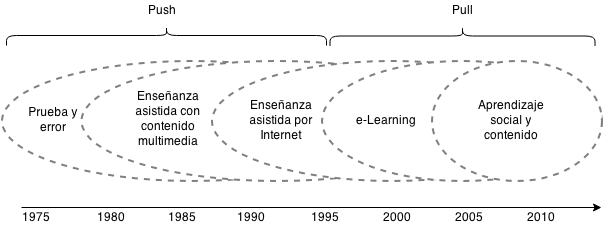
\includegraphics[scale=0.75]{tics/images/tics_history.png}
\caption{Utilización de las \Gls{tic} en la educación desde el año $1975$}
\label{fig:history_tics}
\end{figure}

Para entender la historia de las \Gls{tic} en la educación, se presenta el
gráfico~\ref{fig:history_tics}, en el cual se observa la evolución que sufrió la
utilización de las \Gls{tic} como herramienta en la educación. Se observa que se
parte la historia en cinco corrientes definidas, y a la vez, estas corrientes se
agrupan según el mecanismo de obtención de información, las tres primeras
corrientes se denominan \textit{pull} y las siguientes dos se denominan
\textit{push}. 

\textit{Pull} se refiere a que los estudiantes obtenían la
información sin participar en la creación de la misma, las corrientes
pedagógicas que marcan tendencias en esta época son el instruccionismo y el
conductismo\cite{white:ict}.

\textit{Push} es cuando los alumnos son creados activos de
conocimiento\cite{white:ict,leinonen:ict}, en este periodo de tiempo se
intensifica la creación de herramientas basadas en el constructivismo y el
construccionismo. Es importante notar que las pedagogías de la época
\textit{Pull}, mantienen popularidad y siguen evolucionando, solo que a menor
medida\cite{white:ict}.

El gráfico~\ref{fig:history_tics} muestra el solapamiento entre los diversos
mecanismos utilizados, muestra el inicio de la utilización de una herramienta,
pero no su fin, actualmente se sigue utilizando la mayoría de los
enfoques\cite{leinonen:ict}.

Aunque la figura~\ref{fig:history_tics} muestre un progreso lineal de las
corrientes, este progreso no es igual en todo el mundo, y la el grado de
impacto de las \Gls{tic} varia entre países, lo que se conoce como una
\enquote{brecha tecnológica}. Las fechas utilizadas en el
figura~\ref{fig:history_tics} son relacionadas a la evolución en los Estados
Unidos de Norte America.


\subsection{Instruccionismo}

La educación tradicional o instruccionismo se basa en la transferencia de
conocimiento del profesor al alumno, se enfoca más en el profesor, en la
capacidad del mismo, y en el producto final como resultado de un proceso no
interactivo y bien
documentado\cite{igi:instructionism,johnson2005instructionism}. Los mecanismos
tradicionales para probar la efectividad de este tipo de enseñanza son los
exámenes.

El instruccionismo es conocido además como enseñanza sistemática, enseñanza
explícita, enseñanza directa, y enseñanza activa, siempre enfatizando al
profesor\cite{johnson2005instructionism}.

Epistemológicamente se puede observar al instruccionismo como objetivo, pues
considera que el conocimiento es independiente del entorno, se asume que el
mismo es isomorfo, si el profesor puede enseñar, el alumno puede
aprender\cite{johnson2005instructionism}.

En el instruccionismo, la utilización de las \Gls{tic} en la actualidad se
centra principalmente en mecanismos para proveer contenido, hoy en día se
utilizan plataformas complejas que permiten a los profesores distribuir
contenido y otras actividades relacionadas, estas plataformas se centran bajo
el nombre de \emph{E-Learning}.


\subsubsection{E-Learing} 

El \emph{E-Learning} se define como la educación y capacitación a través de
medios digitales, incluye todo tipo de medio capaz de distribuir información,
puede ser de en tiempo real como salas de conversaciones y videoconferencias o
puede ser diferido, como por ejemplo foros, enciclopedias. Es particularmente
útil para educación a distancia y con horarios flexibles. Se originó a finales
de la década de $1990$ y tuvo su apogeo a mediados de la década del $2000$,
apoyada por la gran penetración de las \Gls{tic} en la
población\cite{punie:ict}.

Se distribuye contenido masivamente a los alumnos, y luego, de manera discreta
se permite a los mismos colaborar, dejando siempre en claro que primero se debe
asimilar toda la información posible y luego relacionarse con los
demás\cite{leinonen:ict}.


\begin{figure}[h] 
\centering 
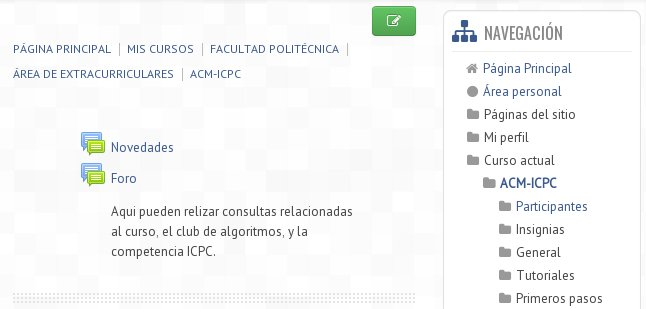
\includegraphics[scale=0.5]{tics/images/moodle.jpg}
\caption{Moodle, plataforma de e Learning} 
\label{fig:moodle}
\end{figure}


La plataforma \emph{Moodle} (ver~\ref{fig:moodle}) cuya primera versión salió en
el $2002$, es una de las principales herramientas del \emph{e-Learning} hoy en
día, permite la creación de cursos específicos por materia y sitios
especializados por instituciones académicas\cite{perkins2006using}. 

La utilización del \emph{e-Learning} tiene varios grados de aplicación en
entornos reales\cite{punie:ict}, que van desde ser simples elementos
complementarios a la clase, como por ejemplo un repositorio para las
diapositivas y otros materiales de clase, hasta cursos completamente en línea,
donde la clase ha sido completamente sustituida.

Sí bien, el \emph{e-Learning} permite la distribución y colaboración en
distintos niveles, no hace un enfoque en el aspecto pedagógico, y se centra en
la forma de transmitir información, y no como la recibe el
alumno\cite{leinonen:ict}, tampoco se centra en la reacción del alumno ante la
información recibida, lo que sí es estudiado por el
conductismo\cite{weegar2012comparison}.

\subsubsection{Conductismo}

El conductismo es una corriente de la psicología, creada por \textit{Jhon
    Watson}, y posteriormente perfeccionada por \textit{Pavlov},
\textit{Skinner}, y \textit{Thorndik}. El conductismo defiende la idea de que
todas las acciones que realizan los seres vivos son consecuencia de un
estímulo. Un ejemplo de esta técnica es el experimento de \textit{Pavlov},
donde un perro es alimentado cada vez que suena una campana, provocando que el
perro salive cuando suena la campana, incluso si no existe una recompensa
(alimento)\cite{weegar2012comparison}.

El conductismo permite a la epistemología utilizar un enfoque científico,
permitiendo controlar todas las variables controlables, como el estímulo y la
reacción, e ignorando los pensamientos y experiencias de las personas (variables
no controladas)\cite{weegar2012comparison}.

La primera incursión del conductismo con las \Gls{tic}, fue presentada por
\textit{Skinner}, en $1958$\cite{weegar2012comparison}, donde se describe una
máquina que contiene botones y una pantalla donde se presenta una pregunta,
para responder el usuario dispone de varias opciones, cada opción esta
relacionada con un botón, si el aprendiz no presiona el botón correcto, debe
seguir intentando hasta acertar y así avanzar\cite{weegar2012comparison}, este
es el inicio de lo que se conoce como \enquote{Prueba y Error}.

Una característica del conductismo, es la ley de \textit{Thorndike}, indica que
una acción cuya consecuencia es un estímulo favorable, es más probable que sea
repetida\cite{weegar2012comparison}, en la
tabla~\ref{tab:conductismo_estimulo}, se observa los distintos mecanismos 
que propone el conductismo para alentar o desalentar un comportamiento.

\begin{table}[!hbt]
\begin{center}
\begin{tabulary}{\textwidth}{|L|C|C|}
\hline
& Comportamiento alentado & Comportamiento reprimido \\
\hline
Estímulo presente & Refuerzo positivo, por ejemplo, buenas notas & Castigo
Presente, por ejemplo, tiempo después de clase \\
\hline
Estímulo eliminado & Refuerzo negativo, por ejemplo, no hacer quehaceres &
Castigo eliminado, por ejemplo, no permitir utilizar la computadora. \\
\hline
\end{tabulary}
\end{center}
\caption{Tipos de estímulos}
\label{tab:conductismo_estimulo}
\end{table}

A finales de la década de $1970$ e inicios de la década de $1980$,  la
complejidad técnica de las computadoras limitaba la cantidad de herramientas
disponibles, los programas eran desarrollados por profesores, y su objetivo era
que los alumnos puedan poner en práctica lo aprendido en el aula. 


El campo de aplicación de las herramientas, basadas en el experimento de
\textit{Skinner}, se limitaban a matemáticas y lenguaje, donde se podía evaluar
inmediatamente los resultados proveídos por los alumnos, pues, normalmente era
un enunciado y una lista posible de opciones del tipo \enquote{Prueba y
    Error}\cite{leinonen:ict}. 

La cantidad limitada de opciones para responder, provocó que los alumnos no
interpreten los resultados, sino prueben todas las posibles opciones hasta
pasar al siguiente enunciado, sin obtener ningún aprendizaje
significativo\cite{leinonen:ict}.

Cuando aparecieron en el mercado computadoras con multimedia, a finales de la
década de $1980$, la utilización de las \Gls{tic} se simplificaron y dieron
contenido a la posibilidad de incluir contenido multimedia, se argumentó que los
ejercicios de tipo \enquote{Prueba y Error} no cumplieron su objetivo de una
educación profunda por que no contenían multimedia\cite{leinonen:ict}, así, en
se empezaron a distribuir las aplicaciones por \textit{CD-ROM} y contener gran
cantidad de contenido multimedia.

Con la creación de los juegos del tipo \enquote{Prueba y Error} y el contenido
multimedia, se inicio a un nueva corriente denominada \emph{Edutainment},
palabra que representa la unión de la educación y el entretenimiento. 

\subsubsection{Edutainment}
\label{sec:edutainment}

Los \emph{edutainment} se basan principalmente en el conductismo y el
cognoscitivismo, se enfoca en juegos sencillos que transmiten información simple
al usuario, su estructura se basa en un objetivo claro que está separado de la
experiencia educativa\cite{egenfeldt2007third}. 

Así el \emph{edutainment} pretende agregar entretenimiento a la educación, se
ve al alumno como un receptor pasivo de información que debe asimilarla, y para
aumentar la implicación de los alumnos, el entretenimiento era
agregado\cite{resnick:2004}.

\emph{Math Blaster} (ver~\ref{fig:math_blaster}) es un \emph{edutainment} donde
el alumno debe responder repetitivamente preguntas aritméticas para obtener
municiones, luego con esas municiones debe completar diferentes misiones en una
nave\cite{bruckman1999can}. Como todas las preguntas se responden mediante un
mecanismo de selección múltiple, y no existe penalización por fallar una
respuesta, los alumnos no reflexionan sobre las respuestas elegidas, seleccionan
una opción aleatoria y si no es la correcta, prueban otra, tras una cantidad
finita de intentos, siempre se obtiene la recompensa deseada.

\begin{figure}[ht!] 
\centering 
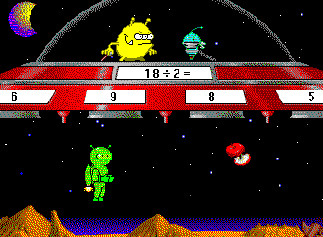
\includegraphics[scale=0.5,natwidth=296,natheight=217]{tics/images/math_blaster.jpg}
\caption{Math Blaster, \emph{edutainment} del año 1987}
\label{fig:math_blaster} 
\end{figure}

\begin{figure}[ht!] 
\centering 
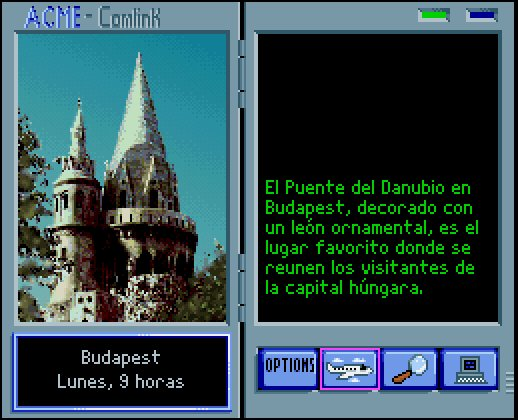
\includegraphics[scale=0.5]{tics/images/carmen.jpg}
\caption{Donde en el mundo esta Carmen Sandiego} 
\label{fig:carmen}
\end{figure}

\enquote{Donde en el mundo esta Carmen Sandiego} (ver~\ref{fig:carmen}) es un
juego que representa el potencial multimedia de esta época, el objetivo del
juego era detener a una serie de criminales mediante varias pistas que eran
provistas en forma de texto. Este exitoso juego demuestra las falencias del
\textit{Edutainment}, siendo visualmente muy atractivo, y con contenido
multimedia acorde a su tiempo, no era más que \enquote{Prueba y Error}, cada
nivel del juego podía ser completado sin leer la información proveída
educativa\cite{charsky:2010}.

Los \emph{edutainment} no logran enseñar habilidades complejas, se enfocan
principalmente en enseñar tareas extremadamente repetitivas que no dependen de
un contexto\cite{charsky:2010,egenfeldt2007third,bruckman1999can}, son
excelentes para enseñar a sumar, pero no para aplicar ese conocimiento, analizar
y obtener conclusiones, o evaluar lo que aprendieron.

Las principales causas por del fracaso de los \emph{edutainment} en su intento
de ser una alternativa viable a la educación son según\cite{egenfeldt2007third}: 

\begin{itemize}

\item \textbf{Falta de motivación interna:} los \emph{edutainment} se centran en
    motivaciones externas, y dejan de lado la motivación interna. Se centran en
    dar recompensas por acciones lo que es una motivación externa, que en que el
    alumno se sienta emocionado al finalizar un nivel, lo que es una forma de
    motivación interna.

\item \textbf{Aprendizaje como anexo:} el principal objetivo del desarrollo de un
    \emph{edutainment} es el de entretener, los objetivos pedagógicos son
    agregados al final. Adicionalmente, este aprendizaje se provee a través de
    largos textos que normalmente son omitidos.

\item \textbf{Interacción limitada:} son construidos con una jugabilidad pobre,
    sin la posibilidad de realizar multiples acciones, normalmente limitados a
    seleccionar respuestas o moverse en un pequeño mundo. 

\item \textbf{Ejercicios de prueba y error sistemáticos:} todas las debilidades
    anteriores se pueden fundamentar en el hecho de que los juegos permiten al
    alumno intentar varias veces sin ser penalizados, además
    de que los alumnos no están motivados, provocaba que todas las opciones sean
    probadas sin el proceso de reflexión necesario para aprender, por ejemplo,
    varios juegos aritméticos solicitaban pruebas del tipo $2+2$ donde el alumno
    probaba diferentes resultados y luego memorizaba el mismo. Se enseñaba a
    probar opciones sin sentido antes que entender y analizar la experiencia.

\end{itemize}

La distribución por medios físicos, aunque contribuyo a la calidad de material
proveído, no resolvió el problema de información actualizada, pues a comienzos
de la década de $1990$, con la popularización de Internet, se genera más
contenido que el que puede ser distribuido por medios físicos, así se accede al
tercer hito de la figura~\ref{fig:history_tics}, donde el contenido es
distribuido por Internet.

La incursión de internet solo permite contenido actualizado, los problemas
persisten y se crean nuevos factores que ensanchan la brecha tecnológica,
ahora, además de poseer una computadora, es necesaria una conexión permanente.
Adicionalmente, la velocidad inicial de Internet no es suficiente para proveer
los mismos entornos ricos en multimedia que sí lo proveían los
CD-ROM\cite{leinonen:ict}.

\textit{Skinner}, se dio cuenta que el compartimiento humano no puede ser
reducido al conductismo, no solo responde a los estímulos, sino, que además
responde a su experiencia previa\cite{weegar2012comparison}, así se estudia el
constructivismo, que se centra en el alumno y sus experiencias.

\subsubsection{Constructivismo}

El constructivismo es una corriente pedagógica creada por \textit{Jean Piaget}
y \textit{Lev Vygotsky}, cuya idea central es que el aprendizaje humano se
construye, que la mente de las personas elabora nuevos conocimientos a partir
de la base de enseñanzas anteriores. Predica que el aprendizaje de los
estudiantes debe ser activo, deben participar en actividades en lugar de
permanecer de manera pasiva observando lo que se les
explica\cite{hernandez:constructivismo,johnson2005instructionism}.

El constructivismo es un conjunto de prácticas que se enfocan en el alumno,
basados en el contenido, orientados al proceso, interactivos y que responden a
las necesidades e intereses personales de los
alumnos\cite{johnson2005instructionism}.

Se basa en que las personas no entienden, ni utilizan de manera inmediata la
información que se les proporciona, en cambio, el individuo debe
\enquote{construir} su propio conocimiento. El conocimiento se construye a
través de la experiencia y esto conduce a la creación de esquemas. Los esquemas
son modelos mentales que almacenamos en nuestras mentes. Estos esquemas van
cambiando, agrandándose y volviéndose más sofisticados a través de dos procesos
complementarios: la asimilación y el
alojamiento\cite{hernandez:constructivismo,johnson2005instructionism}.

Epistemológicamente el constructivismo es subjetivo, pues considera que el
conocimiento depende las experiencias\cite{johnson2005instructionism}. 

Las aulas construccionistas crean un mundo realista donde lo más importante es
el aprendizaje el profesor es un facilitator del aprendizaje del
alumno\cite{johnson2005instructionism,nanjappa2003constructing}.

Actualmente, los cursos de \textit{E-Learing}, tradicionalmente conductistas,
están evolucionando para incluir conceptos
constructivistas\cite{weegar2012comparison}, especialmente donde se requiere de
pensamiento de alto nivel\footnote{Del Inglés, \textit{High Order Thinking},
    incluye la capacidad de resolver problemas complejos, y criterios de
    decisión.}, cuya obtención es vista como una estrategia de actividades
necesarias para conseguir objetivos\cite{miri2007purposely}.

Así, las aplicaciones del constructivismo con las \Gls{tic}, es variado,
incluyendo al \textit{E-Learing} y a los \textit{Edutainment}, hasta lo que hoy
se conoce como \textit{Juegos Serios}, los cuales son descritos en el
capítulo~\ref{chap:juegos_serios}. Otros ejemplos de aplicaciones del
constructivismo, son las \textit{wikis}, redes sociales y los
\textit{blogs}\cite{hernandez:constructivismo}.

Las teoría de \enquote{construccionismo} de \textit{Seymourt Papert},
construida sobre el constructivismo, que agrega, entre otras cosas, la
entorno en la que ocurre el aprendizaje\cite{egenfeldt2007third}, permite
explorar más contenido, proveyendo un punto inicial, y permitiendo explorar
posibles soluciones.
